\documentclass{sosg-informe}

\graphicspath{{../../clima/satelite/figuras/}{figuras/}}
\setlength{\emergencystretch}{1.5em}

\title{Vigilancia satelital GOES-19 de convección profunda\\sobre Santa Cruz (Galápagos):\\evaluación S0 y reglas de vigilancia}
\titulocorto{Vigilancia satelital GOES-19}
\numero{2026-09}
\estado{Borrador para discusión}
\titulocita{Vigilancia satelital GOES-19 de convección profunda sobre Santa Cruz (Galápagos): evaluación S0 y reglas de vigilancia}
\relacionados{PR \issue{85} · repositorio mayait/sosgalapagos-datos}
\date{4 de noviembre de 2026}

\begin{document}
\maketitle

\begin{abstract}
Los modelos globales dieron señal de lluvia fuerte para el 30 de octubre de 2026 con días de antelación, pero no pueden anticipar en qué horas cayó la lluvia intensa que inundó La Cascada (Puerto Ayora). Este informe evalúa si el satélite geoestacionario GOES-19, que ve Galápagos cada 10~min, puede abrir una ventana de vigilancia en las horas previas. Se usaron tres productos de la NOAA: la temperatura de brillo de la banda 13 del ABI, con el umbral de 221~K ($-52$~°C) para los topes de convección profunda y corrección del paralaje; la tasa de lluvia estimada RRQPE; y los rayos del GLM. Se contrastaron con la lluvia medida en Santa Cruz en cuatro eventos, una muestra de 19 días y dos periodos continuos (enero--abril y octubre--2 de noviembre), mediante un cribado horario y un refinamiento a 10~min. La regla de vigilancia v1 (RRQPE $\geq 10$~mm/h a menos de 25~km, o al menos un 10\,\% de la zona con topes por debajo de 221~K, con 3~h de persistencia) se activó 230~min antes de que la regla de lluvia medida llegara al nivel \enquote{medio} en La Cascada y 220~min antes en la parte alta; descontando unos 20~min de latencia quedan unas 3,5~h. Ese adelanto proviene de \textbf{un solo evento convectivo}, con reglas ajustadas después de verlo. Sin RRQPE, detenido por la NOAA desde el 2-nov, el adelanto solo es sólido en la parte alta; en La Cascada depende de 2 imágenes. El satélite no vio las lluvias orográficas \enquote{cálidas} del 3 y el 23-oct. Entre el 1-oct y el 2-nov hubo 5 episodios de vigilancia sin lluvia intensa por zona, y en abril la zona habría estado en vigilancia el 15--18\,\% del tiempo, sin estaciones en la parte alta para saber cuántas veces llovió fuerte. Todo es una estimación satelital y una vigilancia experimental, no una alerta oficial.
\palabrasclave{GOES-19; ABI; topes fríos; paralaje; RRQPE; GLM; convección profunda; vigilancia; alerta temprana; Galápagos.}
\end{abstract}

\begin{aviso}
Este informe presenta \textbf{estimaciones satelitales y reglas propias, no datos oficiales}. La vigilancia satelital es \textbf{experimental}: no es una alerta oficial, no cambia el nivel de inundación calculado con la lluvia medida y no sustituye las indicaciones del COE, la SNGR ni el ECU~911. Se evaluó con \textbf{un solo evento convectivo} (30-oct-2026) y con reglas ajustadas después de verlo, de modo que sus cifras pueden cambiar con el próximo evento. El colector satelital aún no está publicado en el panel de SOS Galápagos y su puesta en marcha requiere aprobación. El análisis lo preparó un equipo asistido por agentes de inteligencia artificial, sin visitas de campo ni revisión profesional externa, y no expresa una posición institucional de la USFQ. Usa datos de GOES-19 de la NOAA (dominio público), lluvia medida del IERSE (CC BY-NC-ND 4.0) y del INAMHI, lluvia diaria de la FCD (CC BY-NC-SA) y una estación particular; los productos derivados de esas series quedan sujetos a sus licencias y al permiso de sus titulares.
\end{aviso}

% =====================================================================
\section{Introducción}

El 30 de octubre de 2026 un sistema convectivo sobre la parte alta de Santa Cruz dejó 61--70~mm en una hora y hasta 240~mm en el día en las estaciones de la red IERSE-WSN, e inundó por la noche el sector de La Cascada, en Puerto Ayora \citep{sosg202602}. El consenso de modelos globales del pronóstico experimental de SOS Galápagos daba \enquote{señal alta} de lluvia fuerte para ese día desde cuatro días antes, pero esos modelos no pronostican la intensidad en 1--3~h \citep{sosg202608}. La regla de nivel por lluvia medida (v0.2) llegó a \enquote{medio} a las 15:10 y a \alto{} a las 15:50, unas cinco horas antes de la llegada modelada del agua al centro de La Cascada \citep{sosg202607,sosg202602}; pero solo reacciona cuando la lluvia ya está cayendo en los pluviómetros.

Entre esas dos escalas, días y minutos, queda un hueco de algunas horas. El satélite GOES-19 (GOES-East, 75,2°~O) observa Galápagos en disco completo cada 10~min y puede ver nacer y crecer los topes de nube muy fríos de la convección profunda antes de que descarguen \citep{schmit2017}. Este informe documenta la \emph{evaluación S0} de esa señal, sus reglas de vigilancia y su operación en tiempo real. Las preguntas son tres:
\begin{enumerate}
  \item ¿Con cuánta anticipación respecto del nivel \enquote{medio} se habría visto la convección del 30-oct?
  \item ¿Qué lluvias fuertes no ve el satélite?
  \item ¿Con qué frecuencia la zona estaría en vigilancia sin que llueva fuerte?
\end{enumerate}

La señal satelital se plantea como complemento: el pronóstico \citep{sosg202608} mira los próximos días; el satélite, las horas previas; y la regla de lluvia medida \citep{sosg202607}, cuya respuesta a tormentas sintéticas se evaluó en el Informe técnico 2026-02 \citep{sosg202602}, el presente.

% =====================================================================
\section{Área de estudio y datos}

\subsection{Zonas evaluadas}
Se evaluaron dos zonas de Santa Cruz, definidas como cajas en \texttt{clima/recolector/zonas\_geo.json} con los mismos identificadores que la regla de lluvia medida:
\begin{itemize}
  \item \textbf{La Cascada} (\texttt{la-cascada}): unos $6 \times 10$~km entre la cuenca alta y Puerto Ayora; unos 15 píxeles de la banda 13.
  \item \textbf{Parte alta de Santa Cruz} (\texttt{santa-cruz-alta}): unos $22 \times 13$~km alrededor de Bellavista y Santa Rosa.
\end{itemize}
Las dos zonas se solapan y comparten estaciones, así que \textbf{no son dos pruebas independientes}. San Cristóbal e Isabela no se evaluaron porque no había estaciones con las que contrastar en los eventos; el colector calcula sus variables, pero las marca \enquote{sin evaluar}.

\subsection{Datos satelitales (estimación satelital)}
Se usaron tres productos de nivel 2 de GOES-19 del archivo abierto de la NOAA \citep{noaa_goes19}, todos en UTC:
\begin{itemize}
  \item \textbf{ABI, banda 13} (10,3~µm, CMIP de disco completo, ${\approx}\,2$~km): temperatura de brillo ($T_b$), que en nubes gruesas se aproxima a la del tope \citep{schmit2017}.
  \item \textbf{ABI, RRQPE}: tasa de lluvia \emph{estimada} por la NOAA a partir del infrarrojo (mm/h, ${\approx}\,2$~km), del linaje del algoritmo SCaMPR \citep{kuligowski2002}. Satura en 100~mm/h.
  \item \textbf{GLM}: destellos de rayos detectados desde el espacio, en archivos de 20~s \citep{goodman2013}.
\end{itemize}
No se guardan netCDF completos: \texttt{goes.py} lee por rangos solo los bloques del recorte de Galápagos (tabla~\ref{tab:productos}). La evaluación S0 bajó en total unos 10~GB con un enlace de ${\approx}\,1$~MB/s desde Galápagos.

\begin{table}[ht]
  \centering\small
  \caption{Productos de GOES-19 y volumen leído por rangos (\texttt{clima/satelite/LEEME.md}).}
  \label{tab:productos}
  \begin{tabular}{lccc}
    \toprule
    Producto & Archivo completo & Lo que se baja & Frecuencia \\
    \midrule
    ABI banda 13 (CMIP, disco completo) & ${\approx}\,24$~MB & ${\approx}\,1,3$~MB & 10~min \\
    ABI RRQPE & ${\approx}\,1,4$~MB & ${\approx}\,0,5$~MB & 10~min \\
    GLM (LCFA) & ${\approx}\,320$~KB cada 20~s & ${\approx}\,55$~KB por archivo & 20~s \\
    \bottomrule
  \end{tabular}
\end{table}

\textbf{Control de calidad.} En el colector se descartan los píxeles de la banda 13 con DQF $\geq 2$, los bits de dato inválido del RRQPE y los destellos con \texttt{flash\_quality\_flag} distinto de 0. La caché de los tres eventos de referencia, de la muestra y de los cribados horarios se bajó antes de añadir esas máscaras y solo descarta el valor de relleno; el refinamiento a 10~min de octubre y de enero--abril sí las aplica.

\subsection{Lluvia medida}
La referencia es la lluvia medida de la tabla de observaciones de la base del recolector de clima, leída en modo de solo lectura:
\begin{itemize}
  \item \textbf{IERSE-WSN} \citep{ierse2023}: Santa Rosa, Los Guayabillos, Cerro Crocker y Militar, cada 5~min desde el 23-abr-2026.
  \item \textbf{INAMHI} M0191, Puerto Ayora \citep{inamhi2026}: horaria hasta el 2-nov; la hora de origen es la continental (UTC$-5$).
  \item \textbf{Estación particular} en la costa de Puerto Ayora.
  \item \textbf{FCD}, Puerto Ayora \citep{fcd2026}: lluvia diaria, la única referencia para enero--abril, cuando aún no había estaciones IERSE.
\end{itemize}
Todas las horas se guardan en UTC y en este informe se dan en hora de Galápagos (UTC$-6$).

\subsection{Eventos y periodos}
\begin{itemize}
  \item \textbf{Cuatro eventos} a 10~min: 30-oct (convectivo, el de la inundación), 23-oct y 3-oct (lluvias orográficas) y 1--2-nov (sin GLM; RRQPE solo hasta el 2-nov a las 10:50).
  \item \textbf{Muestra} de 19 días de mayo a octubre (8 secos, 6 moderados y 5 de lluvia fuerte), con el ABI cada 30~min.
  \item \textbf{Vigilancia continua}: 1-oct a 2-nov y enero--abril de 2026, con el método de la sección~\ref{sec:cribado}.
\end{itemize}

% =====================================================================
\section{Métodos}

\subsection{Topes fríos de convección profunda}
Un tope de nube por debajo de 221~K ($-52$~°C) indica convección profunda; es el umbral de núcleo frío que \citet{maddox1980} usó para los complejos convectivos de mesoescala. Para cada imagen y zona $Z$ se calcula la fracción fría
\begin{equation}
  f_{221}(t) = 100\, \frac{\#\{\, p \in Z : T_b(p,t) < 221~\text{K} \,\}}{\#\{\, p \in Z : T_b(p,t)\ \text{válida} \,\}}\ \ \text{\%},
  \label{eq:frio}
\end{equation}
donde los píxeles $p$ están en su posición corregida por paralaje. También se guardan la $T_b$ mínima de la zona y la fracción en la zona ampliada 25~km.

\subsection{Corrección del paralaje}
Desde 75,2°~O, Galápagos se ve con un ángulo cenital $\theta \approx 18$°. Un tope alto aparece desplazado en sentido contrario al punto subsatelital, es decir, hacia el oeste \citep{vicente2002}. La altura del tope se aproxima a partir de su $T_b$ con el gradiente de la atmósfera estándar \citep{ussa1976}:
\begin{equation}
  h(T_b) = \operatorname{clip}\!\left(\frac{300~\text{K} - T_b}{6,5~\text{K/km}};\ 0;\ 16\right)\ \text{km},
  \label{eq:altura}
\end{equation}
lo que da unos 12~km para 221~K y 15~km para 200~K. \texttt{goes.corregir\_paralaje()} sigue la línea de visión desde el punto observado $\mathbf{P}$ hacia el satélite $\mathbf{S}$ sobre una Tierra esférica de radio $R$:
\begin{equation}
  \mathbf{u} = \frac{\mathbf{S}-\mathbf{P}}{\lVert \mathbf{S}-\mathbf{P} \rVert}, \qquad
  \mathbf{C} = \mathbf{P} + \frac{h}{\mathbf{u}\cdot\mathbf{n}}\,\mathbf{u}, \qquad
  \mathbf{G} = R\, \frac{\mathbf{C}}{\lVert \mathbf{C} \rVert},
  \label{eq:paralaje}
\end{equation}
donde $\mathbf{n} = \mathbf{P}/R$ es la normal local, $\mathbf{C}$ el tope en tres dimensiones y $\mathbf{G}$ el punto de la superficie bajo él. El desplazamiento es aproximadamente $h \tan\theta$: un tope de 14~km se ve unos 4,5~km al oeste de su sitio. El RRQPE se reubica con la altura de la banda 13 del mismo barrido. La corrección importa en La Cascada, de unos 15 píxeles: sin ella, el 30-oct no se veía ningún tope frío sobre la zona antes del \enquote{medio}. La versión sin corrección se reproduce con \texttt{s0\_evaluar.py --sin-paralaje}.

\subsection{Lluvia estimada (RRQPE) y rayos (GLM)}
Se comparó el RRQPE con cada pluviómetro en tres escalas: media horaria en el píxel de la estación y máximo en ventanas de $3\times3$ y $5\times5$ píxeles (${\approx}\,6$ y ${\approx}\,10$~km). Se calcularon el total del evento, el máximo horario, la hora del máximo y la correlación de Pearson horaria. Los destellos del GLM se cuentan por zona en intervalos cerrados de 10~min (30 archivos de 20~s) y en ventanas de 30~min.

\subsection{Señales candidatas y regla de vigilancia v1}
Se probaron nueve señales en tres anillos (zona, 25 y 50~km): $\geq 1$ y $\geq 5$ destellos en 30~min; $f_{221} \geq 10$\,\%; $\geq 25$\,\% de la zona por debajo de 235~K; $T_b$ mínima $\leq 210$~K; RRQPE máximo $\geq 5$, 10 y 20~mm/h; y RRQPE medio $\geq 5$~mm/h. La primera regla combinada (v0) usaba rayos a 25~km, topes fríos a 25~km y RRQPE en la zona, y no daba adelanto frente al \enquote{medio} del 30-oct. Se cambió por la v1 \emph{después de ver ese evento}. La v1, implementada en \texttt{vigilancia.py}, se dispara en el instante $\tau$ si se cumple una de dos condiciones:
\begin{equation}
  D(\tau) = \bigl[\,\mathrm{RRQPE}^{\max}_{25\,\text{km}}(\tau) \geq 10~\text{mm/h}\,\bigr] \ \lor\ \bigl[\,f_{221}(\tau) \geq 10~\text{\%}\,\bigr],
  \label{eq:v1}
\end{equation}
y la zona está en vigilancia mientras haya habido un disparo en las 3~h previas:
\begin{equation}
  V(t) = \max_{\tau \in [\,t-3~\text{h},\ t\,]} D(\tau).
  \label{eq:persistencia}
\end{equation}
Los rayos no entran en la v1: nunca adelantaron nada y casi no hay en Galápagos (sección~\ref{sec:rayos}).

En tiempo real, cada zona toma uno de cinco estados (tabla~\ref{tab:estados}). Un producto \enquote{falta} si su último dato tiene más de 35~min (25~min de vigencia más los 10~min que dura el barrido).

\begin{table}[ht]
  \centering\small
  \caption{Estados de la vigilancia satelital por zona (\texttt{clima/satelite/vigilancia.py}). Ninguno cambia el nivel de inundación.}
  \label{tab:estados}
  \begin{tabularx}{\linewidth}{l>{\raggedright\arraybackslash}X}
    \toprule
    Estado & Significado \\
    \midrule
    \texttt{vigilancia} & Alguna condición de la v1 en las últimas 3~h; se informan el último disparo y la hora hasta la que dura. \\
    \texttt{sin señal} & ABI y RRQPE al día y ninguna condición. No descarta lluvia cálida. \\
    \texttt{incompleta} & Sin disparo, pero falta un producto (hoy, RRQPE): no se puede decir \enquote{sin señal}. \\
    \texttt{sin datos} & No llega ningún producto. \\
    \texttt{sin\_evaluar} & San Cristóbal e Isabela: se muestran los datos, no un estado. \\
    \bottomrule
  \end{tabularx}
\end{table}

\subsection{Referencia, adelanto y latencia}
La referencia es la regla de nivel por lluvia medida v0.2 \citep{sosg202607}, aplicada tal cual con el código del recolector (\texttt{clima/recolector/\allowbreak inundacion.py}) pero sin su persistencia, y evaluada cada 10~min sobre el máximo ponderado de las estaciones válidas de la zona. El nivel \enquote{medio} se alcanza con 15~mm en 1~h, 30~mm en 3~h o 50~mm en 24~h. Sean $t_{\text{medio}}$ y $t_{\text{alto}}$ los primeros instantes en esos niveles. El satélite solo es útil si avisa \emph{antes} de $t_{\text{medio}}$. Si $t_0$ es el inicio del episodio de vigilancia activo en $t_{\text{medio}}$:
\begin{equation}
  A = t_{\text{medio}} - t_0, \qquad A_{\text{ef}} = \max(A - L,\ 0), \qquad L \approx 20~\text{min},
  \label{eq:adelanto}
\end{equation}
donde $L$ es la latencia típica hasta el panel: unos 10~min hasta que el barrido llega al archivo de la NOAA (9,7--10,3~min medidos), hasta 5~min del temporizador del colector y hasta 5~min de la exportación. En total, de 15 a 25~min. Para comparar con la versión 1 de la evaluación, las señales sueltas se miden también sin persistencia, uniendo disparos separados por huecos de hasta 60~min.

\subsection{Cribado horario y refinamiento a 10 min}\label{sec:cribado}
Bajar la banda 13 y el RRQPE cada 10~min durante meses exigiría unos 40~GB. Como la v1 solo puede dispararse con topes muy fríos (el RRQPE también es infrarrojo), \texttt{s0\_cribado.py}:
\begin{enumerate}
  \item mira la banda 13 cada hora (imagen de las HH:00);
  \item marca como candidata cada hora con $T_b$ mínima $< 235$~K a menos de 50~km de las zonas;
  \item alrededor de cada candidata ($\pm 60$~min) baja la banda 13 y el RRQPE cada 10~min.
\end{enumerate}
Fuera de esas ventanas se supone que la v1 no se dispara. En octubre--2-nov hubo 125 horas candidatas de 784, en 17 ventanas, con 148~h a 10~min. En enero--abril, 434 de 2\,872, en 53 ventanas, con 519~h a 10~min.

\subsection{Análisis por episodios y métricas}
Un \emph{episodio de lluvia intensa} es un tramo con $R_{1h} \geq 15$~mm o $R_{3h} \geq 30$~mm en la lluvia medida, uniendo tramos separados por menos de 6~h. Se considera \emph{detectado} si hubo vigilancia entre 6~h antes de su inicio y su final. Un \emph{episodio de vigilancia sin lluvia intensa} es uno que no se solapa con ninguno de esos tramos. Para la cuenta día a día de octubre se usan la probabilidad de detección y la razón de falsas alarmas \citep{wilks2011}:
\begin{equation}
  \mathrm{POD} = \frac{a}{a+c}, \qquad \mathrm{FAR} = \frac{b}{a+b},
  \label{eq:pod}
\end{equation}
con $a$ aciertos, $b$ días con señal sin lluvia intensa y $c$ fallos.

\subsection{Estaciones dudosas}
Se marcaron las horas en que una estación de Santa Cruz registra 0 mientras otra mide al menos 5~mm, y la última hora con lluvia de cada estación (\texttt{resumen.json}, clave \texttt{estaciones\_dudosas}).

% =====================================================================
\section{Resultados}

\subsection{Los eventos}
La tabla~\ref{tab:eventos} resume la lluvia medida y la respuesta satelital en los cuatro eventos. Solo el 30-oct tuvo topes por debajo de 200~K, RRQPE saturado y rayos. El 3 y el 23-oct no bajaron de 230~K ni en el anillo de 25~km.

\begin{table}[ht]
  \centering\small
  \caption{Eventos evaluados. $R_{1h}$ y $R_{3h}$: máximo ponderado de las estaciones válidas de la zona (lluvia medida, mm). Horas de Galápagos (UTC$-6$). $T_b$ mínima, RRQPE máximo y destellos GLM (estimación satelital) en la zona\,/\,anillo de 25~km, con paralaje corregido. LC: La Cascada; SCA: parte alta.}
  \label{tab:eventos}
  \setlength{\tabcolsep}{3.5pt}
  \begin{tabular}{llccccccc}
    \toprule
    Evento & Zona & $R_{1h}$ & $R_{3h}$ & \enquote{medio} & \alto & \makecell{$T_b$ mín.\\(K)} & \makecell{RRQPE\\(mm/h)} & Rayos \\
    \midrule
    30-oct & LC & 61,0 & 133,0 & 15:10 & 15:50 & 198\,/\,191 & 55\,/\,100 & 3\,/\,36 \\
    30-oct & SCA & 69,6 & 139,2 & 15:00 & 15:20 & 191\,/\,191 & 100\,/\,100 & 10\,/\,39 \\
    23-oct & LC & 23,4 & 36,9 & 04:40 & --- & 243\,/\,231 & 1,0\,/\,2,2 & 0\,/\,0 \\
    23-oct & SCA & 31,2 & 49,2 & 05:20 & 05:40 & 242\,/\,231 & 1,0\,/\,2,2 & 0\,/\,0 \\
    3-oct & ambas & 15,6 & 27,4 & 18:30 & --- & 261--262\,/\,260--261 & 0\,/\,0 & 0\,/\,0 \\
    1--2-nov & LC & 21,1 & 30,1 & (2-nov 08:00)$^a$ & --- & 213\,/\,205 & 17\,/\,45 & sin GLM \\
    1--2-nov & SCA & 15,6 & 23,6 & 1-nov 19:50$^b$ & --- & 211\,/\,205 & 17\,/\,48 & sin GLM \\
    \bottomrule
  \end{tabular}
  \par\vspace{3pt}\raggedright\footnotesize $^a$ La regla ya estaba en \enquote{medio} al empezar la ventana por la lluvia de 24~h del 31-oct; se indica el inicio del episodio intenso. $^b$ Con los umbrales rebajados un 20\,\% por la humedad antecedente; el episodio de lluvia intensa sin rebaja empieza a las 20:10.
\end{table}

\subsection{30-oct: el evento convectivo}
Los topes muy fríos aparecieron sobre la parte alta desde las ${\approx}\,$10:30 (figuras~\ref{fig:mapas} y~\ref{fig:evento30}). Con el paralaje corregido, al menos el 10\,\% de la parte alta tenía topes por debajo de 221~K desde las 11:30, y de La Cascada desde las 12:00. El RRQPE pasó de 10~mm/h a menos de 25~km desde las 11:20. Después hubo una pausa de unas 2~h con topes de 225--255~K. El primer chubasco fuerte en Santa Rosa (14--15~h, 43~mm en 1~h) cayó con topes de ${\approx}\,225$~K, es decir, sin satisfacer la condición de topes fríos. La lluvia máxima (19--21~h, 61--70~mm en 1~h) coincidió con el escudo frío más intenso (191--200~K) y con el RRQPE en su techo de 100~mm/h.

La tabla~\ref{tab:adelanto} da los adelantos. Con la v1 y 3~h de persistencia, la vigilancia empezó a las 11:20: 230~min antes del \enquote{medio} en La Cascada y 220~min antes en la parte alta. Descontando la latencia quedan 210 y 200~min, unas 3,5~h. Frente al \alto, el adelanto efectivo sube a 250 y 220~min. La v0 no daba adelanto frente al \enquote{medio}. Si además se exige lluvia en curso en alguna estación ($R_{1h} \geq 5$~mm), el adelanto desaparece en las dos zonas.

\textbf{Sin RRQPE, que es la situación de hoy, el aviso solo es sólido en la parte alta.} Allí, la condición de topes fríos se cumplió de 11:30 a 12:20, con hasta un 43\,\% de la zona por debajo de 221~K, y da 210~min de adelanto (190 efectivos). En La Cascada se apoya en \textbf{solo 2 imágenes}, las de las 12:00 y las 12:10, con 3 de 20 y 4 de 14 píxeles fríos. Con 3~h de persistencia la vigilancia termina a las 15:10, el mismo minuto del \enquote{medio}. Es un \textbf{caso límite}: con 10~min menos de persistencia no habría adelanto, y sin corregir el paralaje, tampoco.

\begin{table}[ht]
  \centering\small
  \caption{Adelanto de la vigilancia frente al primer \enquote{medio} de la regla de lluvia medida (min). \enquote{Sin persistencia}: señal suelta, uniendo huecos de hasta 60~min. \enquote{Efectivo}: con persistencia menos 20~min de latencia (ecuación~\ref{eq:adelanto}). Fuente: \texttt{resumen.json}, \texttt{reglas\_combinadas} y \texttt{contingencia\_episodios}.}
  \label{tab:adelanto}
  \setlength{\tabcolsep}{3.5pt}
  \begin{tabular}{llcccc}
    \toprule
    Evento & Zona & \makecell{v1 sin\\persistencia} & \makecell{v1 con\\persistencia} & \makecell{v1\\efectivo} & \makecell{Solo topes fríos\\(sin RRQPE), efectivo} \\
    \midrule
    30-oct & La Cascada & 100 & 230 & 210 & 170$^a$ \\
    30-oct & Parte alta & 90 & 220 & 200 & 190 \\
    23-oct y 3-oct & ambas & no avisó & no avisó & --- & --- \\
    2-nov, episodio de las 08:00 & La Cascada & --- & 20 & 0 & --- \\
    1-nov, episodio de las 20:10 & Parte alta & --- & no avisó & --- & --- \\
    \bottomrule
  \end{tabular}
  \par\vspace{3pt}\raggedright\footnotesize $^a$ 190~min con persistencia, apoyados en 2 imágenes; la vigilancia acaba a las 15:10, a la misma hora del \enquote{medio} (caso límite).
\end{table}

\begin{figure}[t]
  \centering
  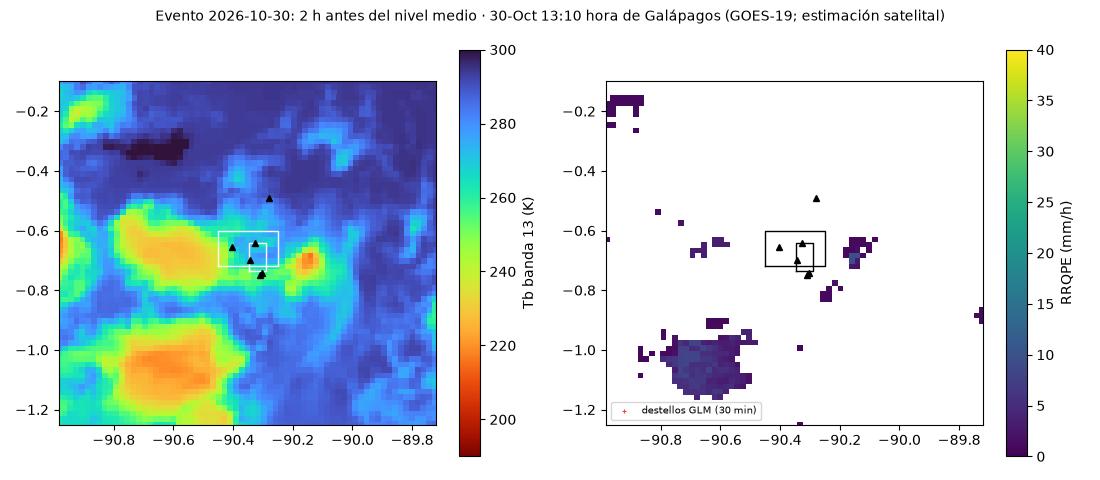
\includegraphics[width=\linewidth]{mapa_2026-10-30_menos2h.png}\\[2pt]
  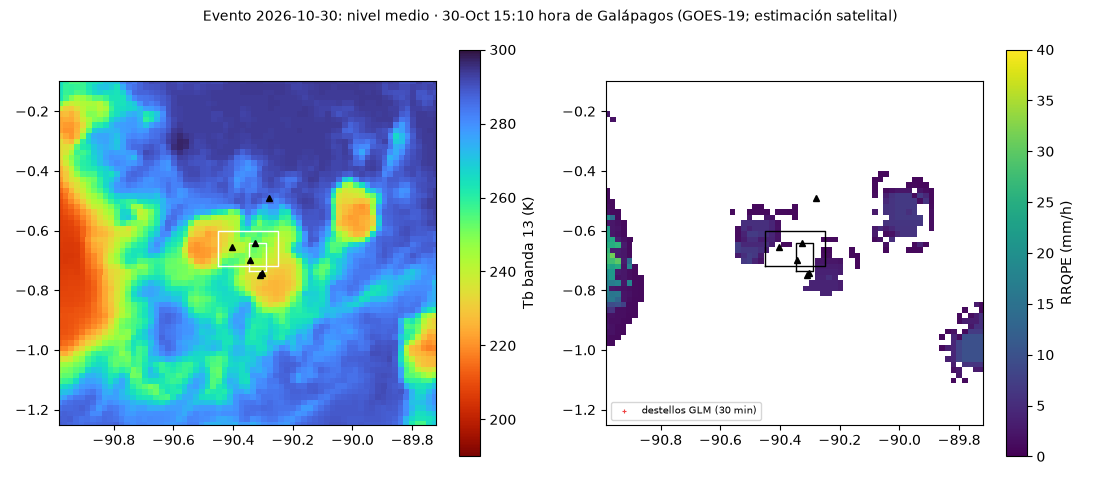
\includegraphics[width=\linewidth]{mapa_2026-10-30_menos0h.png}
  \caption{30-oct-2026 sobre Santa Cruz (estimación satelital). Arriba, a las 13:10, 2~h antes del \enquote{medio} en La Cascada; abajo, a las 15:10, al llegar a \enquote{medio}. Izquierda: $T_b$ de la banda 13 con el paralaje corregido (los tonos naranja y rojo están por debajo de ${\approx}\,225$~K). Derecha: RRQPE (mm/h) y destellos GLM de los últimos 30~min, con las cajas de las dos zonas y las estaciones (\(\blacktriangle\)). La cuadrícula blanca es un artefacto del dibujo de los píxeles reubicados.}
  \label{fig:mapas}
\end{figure}

\begin{figure}[t]
  \centering
  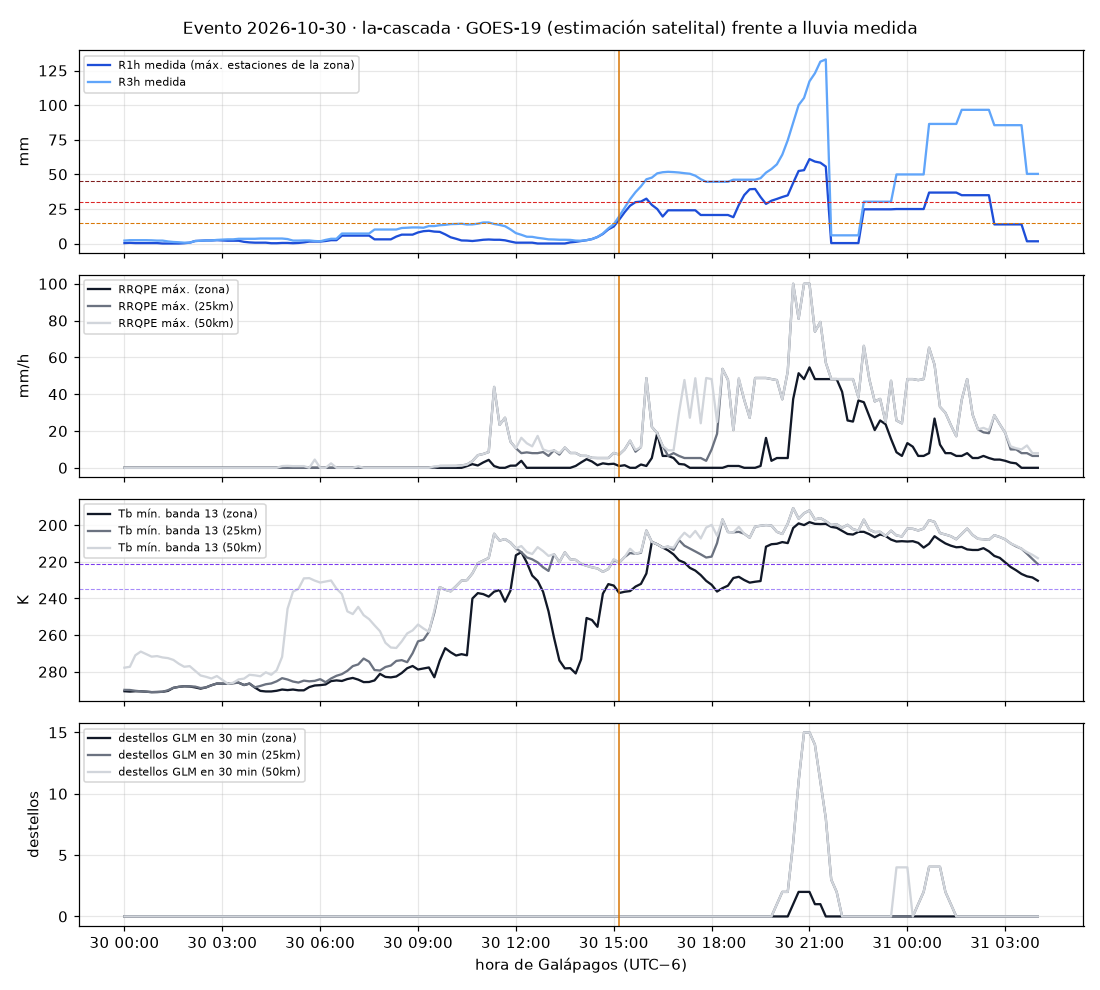
\includegraphics[width=0.82\linewidth]{evento_2026-10-30_la-cascada.png}
  \caption{30-oct-2026, La Cascada. De arriba abajo: $R_{1h}$ y $R_{3h}$ medidos (máximo de las estaciones de la zona; líneas a trazos en 15, 30 y 45~mm); RRQPE máximo en la zona y en los anillos de 25 y 50~km; $T_b$ mínima de la banda 13 (eje invertido; líneas en 221 y 235~K); y destellos GLM en 30~min. La línea vertical marca el primer \enquote{medio} (15:10). Hora de Galápagos.}
  \label{fig:evento30}
\end{figure}

\subsection{3 y 23-oct: lluvia cálida, invisible para el satélite}
El 23-oct, Santa Rosa midió 31~mm en 1~h y la parte alta llegó a \alto{} a las 05:40. El tope más frío sobre la zona fue de 242--243~K (${\approx}\,-30$~°C), el RRQPE no pasó de 2~mm/h y no hubo rayos (figura~\ref{fig:calida}). Los topes se enfriaron poco a poco durante unas 6~h y lo más frío coincidió con la lluvia. El 3-oct, Los Guayabillos midió 68~mm en el día con topes de 261--262~K, RRQPE nulo y sin rayos.

Es lluvia orográfica de nubes bajas y medias: el infrarrojo no puede verla. La misma ausencia de señal aparece en los 5 días de lluvia fuerte de la muestra de mayo a octubre. Por tanto, \textbf{que no haya señal satelital no descarta lluvia fuerte}. En cambio, el consenso de modelos del pronóstico experimental sí daba \enquote{señal alta} para el 23-oct desde cuatro días antes \citep{sosg202608}: pronóstico y satélite se complementan.

\begin{figure}[t]
  \centering
  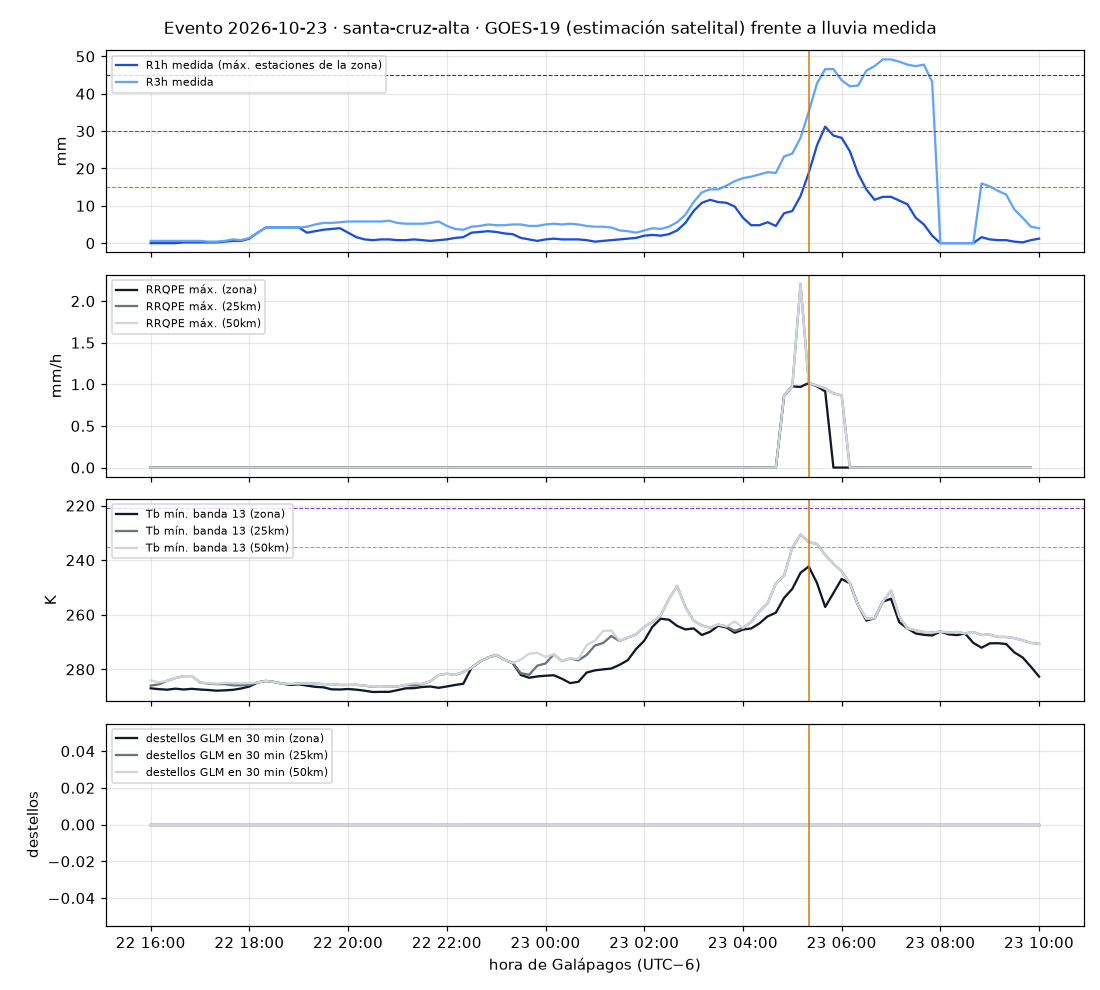
\includegraphics[width=0.495\linewidth]{evento_2026-10-23_santa-cruz-alta.png}\hfill
  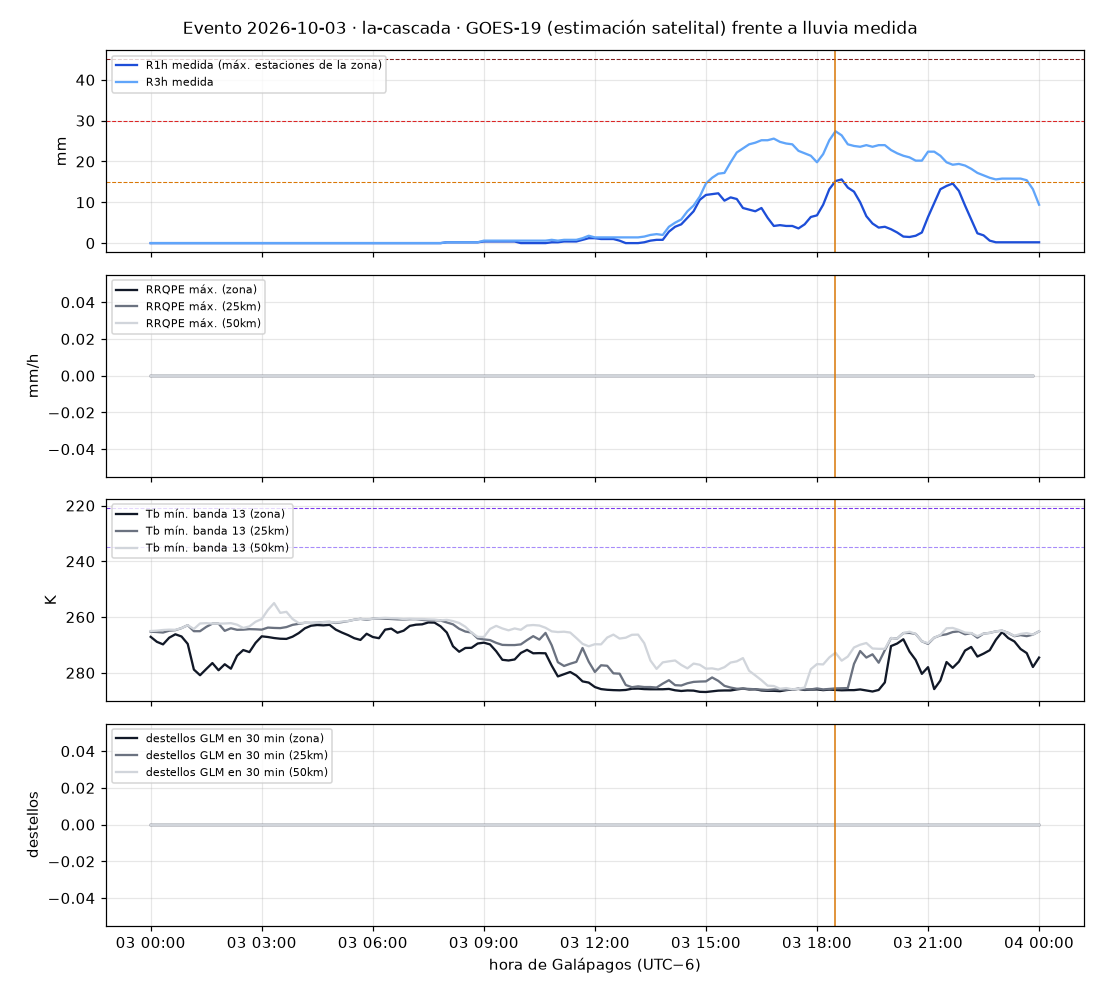
\includegraphics[width=0.495\linewidth]{evento_2026-10-03_la-cascada.png}
  \caption{Lluvias \enquote{cálidas} sin señal satelital. Izquierda: 23-oct, parte alta de Santa Cruz ($R_{1h}$ máximo 31~mm; topes no más fríos que 242~K en la zona; RRQPE $\leq 2,2$~mm/h; sin rayos). Derecha: 3-oct, La Cascada (68~mm en el día en Los Guayabillos; topes de 261--262~K; RRQPE nulo). Mismos paneles que la figura~\ref{fig:evento30}.}
  \label{fig:calida}
\end{figure}

\subsection{1--2-nov}
La v1 se activó varias veces entre la tarde del 31-oct y el 2-nov, con topes de 205--213~K y RRQPE de hasta 45--48~mm/h a 25~km (figura~\ref{fig:nov}). Solo uno de esos episodios precedió a lluvia intensa: el de La Cascada del 2-nov, que empezó a las 08:00 y tuvo vigilancia desde las 07:40, 20~min antes, un adelanto que la latencia anula. El episodio intenso de la parte alta del 1-nov (20:10) no tuvo vigilancia previa. Los demás episodios de vigilancia acompañaron lluvias de 6--11~mm en 1~h.

Dos cautelas afectan a estos días. El RRQPE dejó de producirse el 2-nov a las 10:50, en mitad del periodo. Y Los Guayabillos no registra lluvia desde la noche del 30-oct (sección~\ref{sec:dudosas}): La Cascada se midió solo con el INAMHI y Santa Rosa (peso 0,75), y la parte alta solo con Santa Rosa, de modo que algún episodio \enquote{moderado} pudo ser intenso.

\begin{figure}[t]
  \centering
  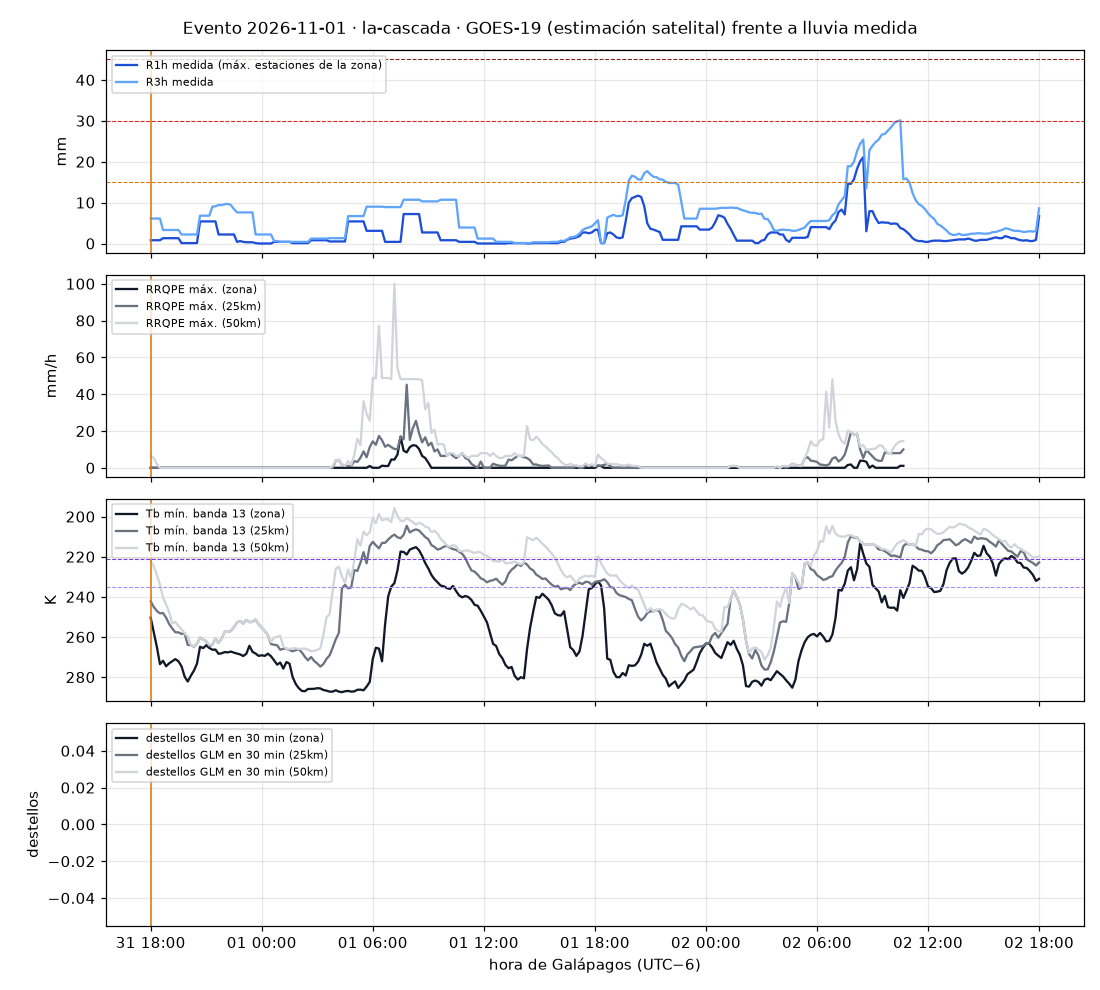
\includegraphics[width=0.74\linewidth]{evento_2026-11-01_la-cascada.png}
  \caption{31-oct a 2-nov-2026, La Cascada. Mismos paneles que la figura~\ref{fig:evento30}; sin datos del GLM en este periodo y sin RRQPE desde el 2-nov a las 10:50. La línea vertical marca el inicio de la ventana, ya en \enquote{medio} por la lluvia de 24~h del 31-oct.}
  \label{fig:nov}
\end{figure}

\subsection{RRQPE frente a los pluviómetros}
En el 30-oct, el RRQPE acertó la hora de máxima lluvia en Santa Rosa y Los Guayabillos (correlación horaria de 0,80--0,81 en $5\times5$), pero subestimó la cantidad: de 4 a 9 veces en el píxel y de 1,6 a 3 veces en el máximo $5\times5$ en Santa Rosa, Los Guayabillos y Puerto Ayora (tabla~\ref{tab:rrqpe}). Puso lluvia donde casi no llovió (Cerro Crocker y Militar). En Puerto Ayora, el pico medido llegó 3~h después del estimado; la hora de origen continental del INAMHI añade incertidumbre a esa diferencia. En la lluvia cálida, el RRQPE dio prácticamente cero. \textbf{No sirve como dato de lluvia}, solo como indicio de convección.

\begin{table}[ht]
  \centering\small
  \caption{RRQPE (estimación satelital) frente a la lluvia medida, con paralaje corregido. Totales del evento y máximos horarios en mm. Fuente: \texttt{resumen.json}, clave \texttt{rrqpe\_vs\_pluviometros}.}
  \label{tab:rrqpe}
  \setlength{\tabcolsep}{3.5pt}
  \begin{tabular}{llcccccc}
    \toprule
    Estación & Evento & \makecell{Total\\medido} & \makecell{RRQPE píxel\,/\\máx. $5\times5$} & \makecell{Máx. 1~h medido\,/\\RRQPE $5\times5$} & \makecell{Misma hora\\pico} & \makecell{$r$ horario\\($5\times5$)} \\
    \midrule
    Santa Rosa & 30-oct & 216,0 & 46,5\,/\,104,4 & 66,4\,/\,55,5 & sí & 0,81 \\
    Los Guayabillos & 30-oct & 153,2 & 16,9\,/\,51,7 & 61,0\,/\,25,8 & sí & 0,80 \\
    INAMHI Puerto Ayora & 30-oct & 205,6 & 48,4\,/\,128,0 & 36,8\,/\,41,3 & no (3~h) & 0,29 \\
    Estación particular & 30-oct & 69,3 & 69,7\,/\,145,9 & 19,2\,/\,42,2 & no (3~h) & 0,39 \\
    Cerro Crocker & 30-oct & 4,8 & 31,1\,/\,92,5 & 0,8\,/\,46,7 & --- & $-0,07$ \\
    Militar & 30-oct & 2,4 & 12,3\,/\,33,3 & 0,8\,/\,7,2 & --- & 0,41 \\
    \addlinespace
    Santa Rosa & 23-oct & 81,0 & 0,0\,/\,0,3 & 28,2\,/\,0,3 & --- & --- \\
    Los Guayabillos & 3-oct & 68,2 & 0,0\,/\,0,0 & 12,6\,/\,0,0 & --- & --- \\
    \bottomrule
  \end{tabular}
\end{table}

\subsection{Rayos}\label{sec:rayos}
El 30-oct hubo 36--39 destellos de calidad buena a menos de 25~km de las zonas (3 dentro de La Cascada y 10 dentro de la parte alta), todos entre las 20:30 y las 21:30, en pleno pico de lluvia. Ninguno antes. En la muestra de mayo a octubre, la señal de al menos un destello en 30~min a 50~km solo apareció en un día moderado. Los rayos acompañan a la convección intensa sobre Santa Cruz, pero llegan tarde y son escasos; por eso salieron de la regla.

\subsection{Falsas alarmas y detección: octubre a 2-nov}
\textbf{Muestra de mayo a octubre.} La v1 no se disparó en ninguno de los 19 días (0 de 8 secos, 0 de 6 moderados y 0 de 5 fuertes). Pero solo 1 de 672 imágenes tenía topes por debajo de 221~K sobre las zonas, así que la muestra apenas pone a prueba la señal. Los días se eligieron con una semilla fija, aunque la regla de selección se escribió a mano.

\textbf{Octubre, día a día.} Con la banda 13 cada hora y la condición $f_{221} \geq 10$\,\% en la zona, La Cascada tuvo 3 aciertos, 2 fallos (3 y 23-oct) y 2 días con señal sin lluvia intensa de 28 (tabla~\ref{tab:octubre}). Esta cuenta mezcla episodios: el \enquote{acierto} del 31-oct es la cola del 30-oct, y el 1 y el 2-nov son un mismo episodio.

\begin{table}[ht]
  \centering\small
  \caption{Octubre de 2026 (y 1--2-nov), día a día, con la banda 13 cada hora. Lluvia intensa: $R_{1h} \geq 15$ o $R_{3h} \geq 30$~mm en el día de Galápagos. POD y FAR según la ecuación~\ref{eq:pod}. Fuente: \texttt{resumen.json}, clave \texttt{octubre}.}
  \label{tab:octubre}
  \begin{tabular}{llcccccc}
    \toprule
    Zona & Señal (imagen horaria) & Días & Aciertos & Fallos & \makecell{Señal sin\\lluvia intensa} & POD & FAR \\
    \midrule
    La Cascada & $f_{221} \geq 10$\,\% (zona) & 33 & 3 & 2 & 2 & 0,60 & 0,40 \\
    La Cascada & $\geq 25$\,\% bajo 235~K (25~km) & 33 & 3 & 2 & 3 & 0,60 & 0,50 \\
    La Cascada & $T_b$ mín. $\leq 210$~K (zona) & 33 & 2 & 3 & 0 & 0,40 & 0,00 \\
    Parte alta & $f_{221} \geq 10$\,\% (zona) & 32 & 2 & 2 & 2 & 0,50 & 0,50 \\
    Parte alta & $\geq 25$\,\% bajo 235~K (25~km) & 32 & 2 & 2 & 3 & 0,50 & 0,60 \\
    Parte alta & $T_b$ mín. $\leq 210$~K (zona) & 32 & 1 & 3 & 0 & 0,25 & 0,00 \\
    \bottomrule
  \end{tabular}
\end{table}

\textbf{Por episodios, con la v1 a 10~min y persistencia} (tabla~\ref{tab:episodios} y figura~\ref{fig:sintesis}b). Se detectaron 2 de 4 episodios de lluvia intensa en La Cascada (30-oct con 230~min y 2-nov con 20~min; solo el primero es útil tras la latencia) y 1 de 4 en la parte alta (30-oct, 220~min). Hubo 5 episodios de vigilancia sin lluvia intensa por zona: dos sin nada de lluvia (24 y 27-oct, de 3 a 4~h cada uno) y tres con lluvia moderada, de 6 a 11~mm en 1~h, el 31-oct y el 1--2-nov. Los días con convección cercana pero sin evento que señaló la revisión independiente (11, 16 y 25-oct) no dispararon la v1. La zona estuvo en vigilancia 29,8~h en octubre en La Cascada (4,0\,\% del mes) y 27,5~h en la parte alta (3,7\,\%); el 1--2-nov, el 31--34\,\% del tiempo.

\begin{table}[ht]
  \centering\small
  \caption{Octubre a 2-nov por episodios (v1 a 10~min con 3~h de persistencia). Detectado: vigilancia entre 6~h antes del inicio del episodio y su final. Fuente: \texttt{resumen.json}, clave \texttt{contingencia\_episodios}.}
  \label{tab:episodios}
  \begin{tabularx}{\linewidth}{l>{\raggedright\arraybackslash}Xcccc}
    \toprule
    Zona & Episodios de lluvia intensa & Detectados & \makecell{Útiles tras\\la latencia} & \makecell{Vigilancia sin\\lluvia intensa} & \makecell{Episodios de\\vigilancia} \\
    \midrule
    La Cascada & 4 (3-oct, 23-oct, 30-oct, 2-nov 08:00) & 2 & 1 & 5 & 7 \\
    Parte alta & 4 (3-oct, 23-oct, 30-oct, 1-nov 20:10) & 1 & 1 & 5 & 6 \\
    \bottomrule
  \end{tabularx}
\end{table}

\begin{table}[ht]
  \centering\small
  \caption{Episodios de vigilancia v1 sin lluvia intensa (hora de Galápagos). Lluvia medida máxima en 1~h durante el episodio.}
  \label{tab:falsas}
  \begin{tabularx}{\linewidth}{lc>{\raggedright\arraybackslash}X}
    \toprule
    Inicio & Duración & $R_{1h}$ máximo medido \\
    \midrule
    24-oct, 10:20--10:30 & ${\approx}\,4$~h & 0~mm (las dos zonas) \\
    27-oct, 03:50 & ${\approx}\,3$~h & 0~mm (solo La Cascada) \\
    31-oct, 14:10 & ${\approx}\,5$~h & 7,6~mm (La Cascada); parte alta sin datos (estaciones cortadas) \\
    1-nov, 05:50 & ${\approx}\,6,5$~h & 7,2~mm (La Cascada)\,/\,0,6~mm (parte alta) \\
    2-nov, 06:30 (parte alta) y 14:20--14:30 & 3,5--5~h & 6,7--11~mm \\
    \bottomrule
  \end{tabularx}
\end{table}

\subsection{Vigilancia continua de enero a abril}
En enero--abril de 2026 la v1 habría estado activa 0~h en enero, 0--6~h en febrero, 26--30~h en marzo (${\approx}\,4$\,\%) y 111--127~h en abril, el 15--18\,\% del mes (tabla~\ref{tab:eneabr} y figura~\ref{fig:sintesis}a). Fueron 24 episodios en La Cascada (5 en marzo y 19 en abril) y 25 en la parte alta, de 3 a 14~h cada uno. Entre el 14 y el 27 de abril la vigilancia fue casi diaria. Abril es la temporada convectiva.

No había estaciones en la parte alta: la red IERSE empieza el 23-abr. La única referencia es la lluvia diaria de la FCD en Puerto Ayora, al nivel del mar. Hubo vigilancia en 18 días en La Cascada y en 22 en la parte alta; 5 de ellos no tienen dato de la FCD. Con dato, solo 3--4 días pasaron de 10~mm en la costa (20-mar, 15-abr con 49~mm y 24-abr) y uno pasó de 20~mm. Al revés, de los 8 días con al menos 10~mm en la FCD entre enero y abril, la v1 estuvo activa en 3--4; los demás, casi todos en febrero, fueron lluvia sin topes fríos. La costa no permite decir cuántos de esos episodios trajeron lluvia intensa a la parte alta, porque la convección suele descargar arriba: \textbf{la tasa real de falsas alarmas en la temporada convectiva no está calculada}.

\begin{table}[ht]
  \centering\small
  \caption{Vigilancia continua con la v1 (cribado horario y refinamiento a 10~min). Horas en vigilancia y porcentaje del mes. Fuente: \texttt{resumen.json}, clave \texttt{vigilancia\_continua}.}
  \label{tab:eneabr}
  \begin{tabular}{lccc}
    \toprule
    Mes (2026) & \makecell{Horas candidatas\\del cribado} & La Cascada & Parte alta \\
    \midrule
    Enero & 0 & 0 (0\,\%) & 0 (0\,\%) \\
    Febrero & 73 & 0 (0\,\%) & 6,3 (0,9\,\%) \\
    Marzo & 98 & 25,8 (3,5\,\%) & 29,5 (4,0\,\%) \\
    Abril & 263 & 110,8 (15,4\,\%) & 126,5 (17,6\,\%) \\
    \addlinespace
    Octubre & \multirow{2}{*}{125 (oct--2-nov)} & 29,8 (4,0\,\%) & 27,5 (3,7\,\%) \\
    1--2 de noviembre & & 14,8 (30,9\,\%) & 16,3 (34,0\,\%) \\
    \bottomrule
  \end{tabular}
  \par\vspace{3pt}\raggedright\footnotesize Mayo a septiembre: no calculado. De los pasos con banda 13 (5\,415 en enero--abril y 1\,925 en octubre--2-nov), 2\,311 y 515 no tienen RRQPE; casi todos son imágenes horarias del cribado, más el final del 2-nov.
\end{table}

\begin{figure}[t]
  \centering
  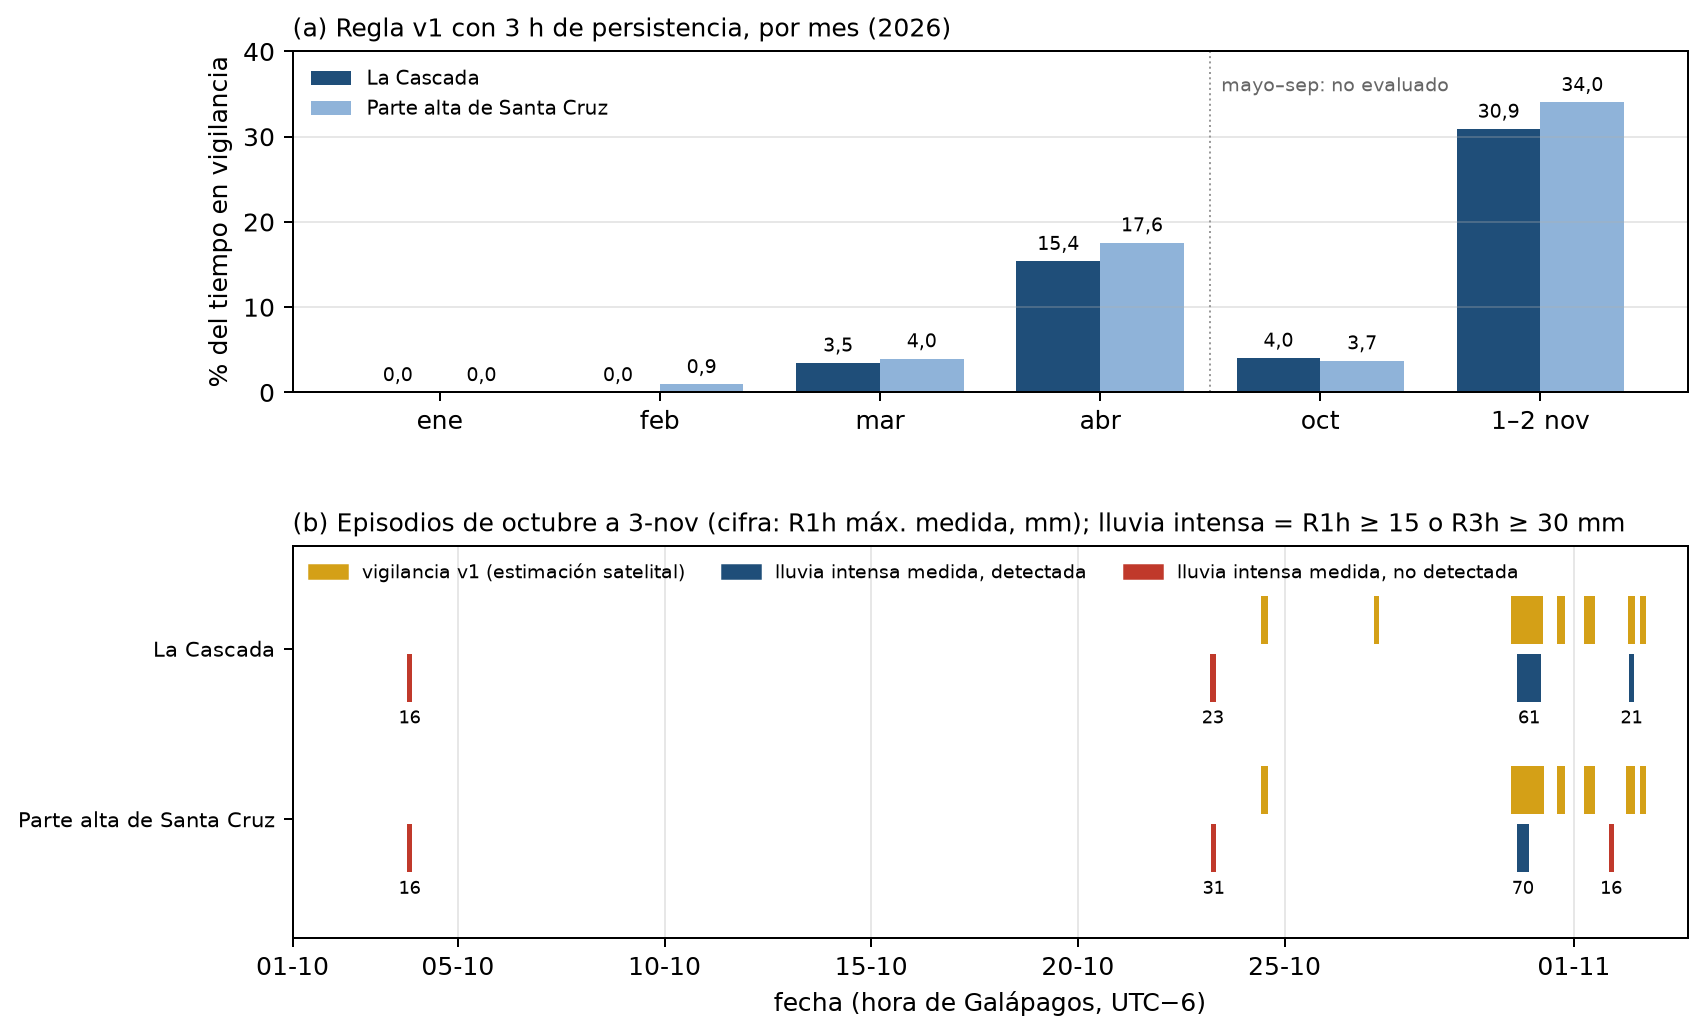
\includegraphics[width=\linewidth]{vigilancia_sintesis.png}
  \caption{Síntesis de la vigilancia v1 (estimación satelital). (a) Porcentaje del tiempo en vigilancia por mes y zona; mayo a septiembre no se calculó. (b) Cronología de octubre a 3-nov: episodios de vigilancia (arriba, ocre) frente a episodios de lluvia intensa medida (abajo; azul si se detectaron, rojo si no), con el $R_{1h}$ máximo medido en mm. Generada por \texttt{informes/2026-09-satelite/figuras.py} a partir de \texttt{clima/satelite/resumen.json}.}
  \label{fig:sintesis}
\end{figure}

\subsection{Estaciones dudosas}\label{sec:dudosas}
\textbf{Los Guayabillos} registró lluvia por última vez el 30-oct a las 20:00 (31-oct, 02:00~UTC). Desde entonces marca 0 mientras Santa Rosa o el INAMHI miden de 7 a 16~mm/h: 4~h el 1-nov, 6~h el 2-nov y 1~h el 3-nov. Parece obstruido, quizá por el propio evento del 30-oct. El 23-oct también marcó 0 durante 5~h con Santa Rosa en 28~mm/h, aunque allí puede tratarse de lluvia muy local. La regla v0.2 ya excluye una estación que marca 0 en 3~h si otra válida mide al menos 10~mm, pero con lluvias de 5--10~mm la excluye tarde o no la excluye. \textbf{Cerro Crocker} marca 0 en horas sueltas con lluvia abajo (garúa y lluvia muy local), sin indicios de obstrucción. Una estación obstruida debilita a la vez la regla de lluvia medida y esta evaluación.

\subsection{Operación en tiempo real}
El colector (\texttt{colector.py}) corre cada 5~min, lee solo los barridos nuevos, corrige el paralaje, aplica las máscaras de calidad y guarda los agregados por zona en la base del recolector. También escribe un archivo público pequeño (10--40~KB) con las últimas 3~h por zona, los destellos, los núcleos fríos y el estado de vigilancia, que viaja dentro del estado general del panel. Cada corrida baja unos 4~MB (${\approx}\,17$~GB al mes) y no guarda ningún netCDF.
\begin{itemize}
  \item \textbf{Latencia:} la banda 13 y el RRQPE llegan al panel con 15--25~min de antigüedad desde el inicio del barrido; el GLM, con 10--20~min, porque se cuenta en intervalos cerrados de 10~min.
  \item \textbf{Robustez:} 15~s de tiempo máximo por petición y 3 intentos; un plazo de 170~s por corrida; lo que no cabe queda para la siguiente, y los fallos se registran como errores de la corrida.
  \item \textbf{Cortes de la NOAA:} la producción de RRQPE se detuvo el 2-nov-2026 a las 10:50 (16:50~UTC), también en GOES-18, y seguía detenida el 4-nov. El colector sigue con la banda 13 y el GLM, y el estado de las zonas pasa a \enquote{incompleta} en lugar de \enquote{sin señal}.
  \item \textbf{Estado:} probado en local en tiempo real y repitiendo el 30-oct. \textbf{No se ha publicado en el panel}; su puesta en marcha requiere aprobación.
\end{itemize}

% =====================================================================
\section{Discusión y limitaciones}

El satélite añade información en una escala de tiempo que ni el pronóstico ni la lluvia medida cubren. El pronóstico experimental \citep{sosg202608} dio \enquote{señal alta} con días de antelación para el 23 y el 30-oct, pero no dice en qué hora lloverá fuerte. La regla de lluvia medida \citep{sosg202607} avisa entre 25~min y 2~h antes de las inundaciones modeladas con tormentas sintéticas \citep{sosg202602}, pero solo cuando la lluvia ya cae. El 30-oct, los topes fríos sobre la parte alta abrieron una ventana de unas 3,5~h antes del \enquote{medio}. Al mismo tiempo, la señal satelital solo ve una de las dos formas en que llueve fuerte en Santa Cruz: la convectiva. Las limitaciones principales son estas:
\begin{itemize}
  \item \textbf{Un solo evento convectivo y reglas ajustadas después de verlo.} La v0 no daba adelanto; la v1 se eligió tras el 30-oct, que es también el único evento con adelanto útil. Hay riesgo real de sobreajuste, y el adelanto de 3,5~h no es una estimación de lo que ocurrirá en el próximo evento.
  \item \textbf{No ve la lluvia cálida.} El 3 y el 23-oct, y los 5 días fuertes de la muestra, pasaron sin señal. \enquote{Sin señal} no significa \enquote{sin lluvia fuerte}, y por eso la vigilancia nunca baja el nivel de inundación.
  \item \textbf{Dependencia del RRQPE.} Los 3,5~h de La Cascada se apoyan en el RRQPE a 25~km. Sin él, detenido desde el 2-nov, el adelanto en La Cascada es un caso límite de 2 imágenes que depende de la corrección del paralaje y de la duración exacta de la persistencia.
  \item \textbf{Falsas alarmas sin medir en la temporada convectiva.} En abril la zona estaría en vigilancia el 15--18\,\% del tiempo, y no hay estaciones en la parte alta para saber cuántos de esos episodios fueron reales. Entre el 1-oct y el 2-nov hubo 5 episodios sin lluvia intensa por zona.
  \item \textbf{Zonas solapadas y solo en Santa Cruz.} La Cascada y la parte alta comparten estaciones. San Cristóbal, que tuvo lluvia intensa el 1 y el 2-nov según el GSC, no se evaluó.
  \item \textbf{Lluvia de referencia frágil.} Los Guayabillos parece obstruido desde el 30-oct; las estaciones de la parte alta dejaron de transmitir hacia las 21:45 del 30-oct; y el INAMHI usa la hora continental.
  \item \textbf{Supuestos del método.} Fuera de las ventanas del cribado se supone que la v1 no se dispara: es razonable, porque exige topes muy fríos, pero no está medido. La altura del tope para el paralaje es una aproximación por $T_b$ (ecuación~\ref{eq:altura}). La caché de los eventos, de la muestra y de los cribados horarios se bajó sin las máscaras de calidad. El RRQPE tiene un techo de 100~mm/h.
  \item \textbf{Latencia.} De 15 a 25~min hasta el panel. El adelanto del 2-nov (20~min) queda anulado.
\end{itemize}

La evaluación S0 (\texttt{clima/satelite/evaluacion-s0.md}) propone usar la señal en dos fases. En la fase A, experimental, la vigilancia se muestra aparte del nivel, en un color neutro, solo en las dos zonas evaluadas, sin subir ni bajar el nivel y con la advertencia de que no ve la lluvia cálida. Si las estaciones callan mientras hay vigilancia satelital, la tarjeta lo diría de forma explícita, como refuerzo de la regla de \enquote{silencio en alerta} ya vigente. Una fase B, en la que la vigilancia adelantaría el \enquote{medio}, queda condicionada en ese documento a al menos 3 eventos convectivos con adelanto evaluados con reglas fijadas \emph{antes} de verlos, una temporada de falsas alarmas a 10~min con el colector en marcha, zonas que no se solapen y la revisión del especialista en gestión de riesgos. Con la evidencia de este informe, los resultados no justifican que la señal satelital cambie el nivel de inundación.

% =====================================================================
\section{Conclusiones y trabajo futuro}
\begin{enumerate}
  \item El 30-oct, la regla v1 habría abierto la vigilancia a las 11:20, unas 3,5~h antes del \enquote{medio} una vez descontada la latencia. Es un solo evento convectivo y las reglas se ajustaron después de verlo.
  \item Sin RRQPE, que la NOAA dejó de producir el 2-nov, el adelanto solo es sólido en la parte alta (190~min efectivos); en La Cascada es un caso límite de 2 imágenes.
  \item El satélite no ve la lluvia orográfica cálida: el 3 y el 23-oct no tuvieron señal. El pronóstico de modelos sí dio señal para el 23-oct: las dos fuentes se complementan.
  \item El RRQPE acierta la hora del pico en la parte alta, pero subestima la lluvia de 4 a 9 veces en el píxel; no es un dato de lluvia. Los rayos llegan con el pico y no adelantan nada.
  \item Entre el 1-oct y el 2-nov hubo 5 episodios de vigilancia sin lluvia intensa por zona, y la vigilancia ocupó ${\approx}\,4$\,\% de octubre; en abril, la vigilancia ocuparía el 15--18\,\% del tiempo, con una tasa de aciertos no calculada.
\end{enumerate}

Para pasar de vigilancia experimental a una señal evaluada hacen falta:
\begin{itemize}
  \item nuevos eventos convectivos evaluados con la v1 congelada;
  \item una temporada completa del colector a 10~min, contrastada con estaciones en la parte alta;
  \item la evaluación de San Cristóbal, con el GSC y el INAMHI, empezando por el 1 y el 2-nov;
  \item probar la tendencia de enfriamiento ($T_b$ que baja más de 20~K en 1~h) como señal más temprana;
  \item revisar Los Guayabillos y vigilar la reanudación del RRQPE.
\end{itemize}

\section*{Disponibilidad de datos y código}
{\small Todo el procesamiento está en el repositorio público \emph{mayait/sosgalapagos-datos}, carpeta \texttt{clima/satelite/}:
\begin{itemize}
  \item \texttt{goes.py} (lectura por rangos, proyección geoestacionaria, máscaras de calidad y corrección del paralaje);
  \item \texttt{colector.py} (colector en tiempo real) y \texttt{vigilancia.py} (regla v1 y estados);
  \item \texttt{s0\_extraer.py}, \texttt{s0\_cribado.py} y \texttt{s0\_evaluar.py} (evaluación S0);
  \item \texttt{resumen.json} (todas las cifras), \texttt{evaluacion-s0.md} (informe de trabajo) y \texttt{figuras/}.
\end{itemize}
La caché de recortes (\texttt{clima/satelite/cache/}) no se versiona; \texttt{s0\_extraer.py} la reconstruye desde el archivo abierto de la NOAA. La lluvia medida procede de la base del recolector de clima, que no es pública. La figura~\ref{fig:sintesis} la genera \texttt{informes/2026-09-satelite/figuras.py}, y este informe se compila con \texttt{informes/compilar.sh 2026-09-satelite}.\par}

\bibliographystyle{sosg}
\bibliography{referencias,bib-2026-09}

\end{document}
